\section{Implementation}

The implementation connects the main experimental activities described in the design section. A researcher can collect or import monitoring data, train several compatible detectors, compare their Saved Models, and continue with Live Monitoring and root-cause analysis (RCA). CloudSentinel stores the identity of the data, model, configuration, and result at every transition. The implementation therefore focuses on connecting the workflow and preserving its evidence, rather than introducing a new anomaly-detection or RCA algorithm.

Figure~\ref{fig:implementation_workflow_overview} shows the main entry point. It presents the lifecycle as one route and suggests a next action based on the artefacts that already exist. The same guide appears on detailed pages. For example, a completed Training Run can open a new Model Comparison with its successful Saved Models already selected. A completed experiment does not leave the application permanently at its final step; the overview also allows a new experiment to start while earlier evidence remains available in history.

\begin{figure}[H]
    \centering
    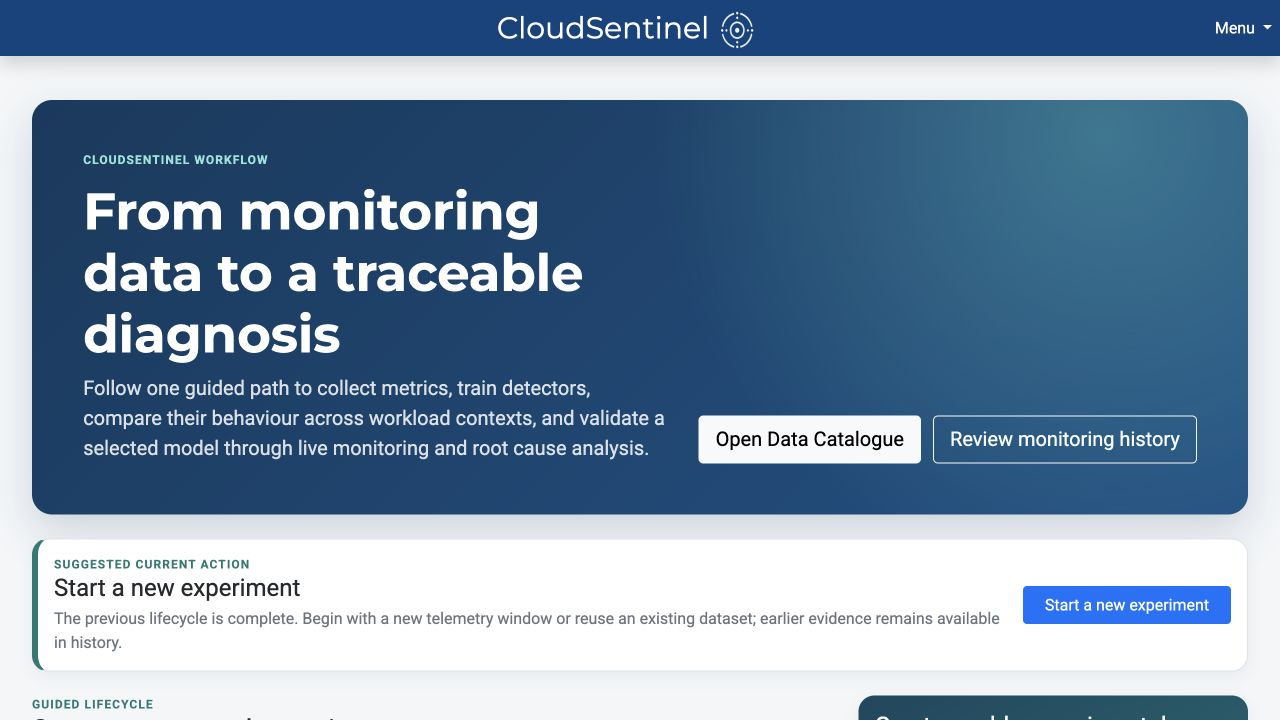
\includegraphics[width=0.95\linewidth]{figures/implementation/current/workflow_overview.jpg}
    \caption{The implemented workflow overview connects dataset collection, training, comparison, monitoring, and stored evidence.}
    \label{fig:implementation_workflow_overview}
\end{figure}

\subsection{Overall implementation structure}

The redesign was implemented inside the existing CloudSentinel services instead of replacing the complete system. Figure~\ref{fig:condensed_implementation_architecture} summarises the responsibilities that are most important for understanding the workflow.

The Django user interface presents the workflow but does not directly read internal files or model artefacts. Dataset operations and Live Monitoring are handled through the Data Ingestion service. Detector discovery, training, Saved Models, and Model Comparisons are handled through the Learning service. Long-running collection, training, comparison, and monitoring work is sent to Celery workers through Redis. The Generic Detection Runtime loads a selected model through its detector adapter and applies the preprocessing stored with that model. The existing CRCA service executes the selected RCA method after Data Ingestion has committed the monitoring evidence that triggered it.

\begin{figure}[H]
    \centering
    \resizebox{0.98\linewidth}{!}{%
    \begin{tikzpicture}[
        font=\small,
        node distance=10mm and 11mm,
        component/.style={draw, rounded corners=2pt, align=center, minimum height=11mm, text width=28mm, fill=blue!7},
        storage/.style={draw, cylinder, shape border rotate=90, aspect=0.25, align=center, minimum height=14mm, text width=27mm, fill=green!10},
        external/.style={draw, rounded corners=2pt, align=center, minimum height=11mm, text width=25mm, fill=orange!11},
        flow/.style={-{Latex[length=2mm]}, thick},
        evidence/.style={-{Latex[length=2mm]}, thick, dashed}
    ]
        \node[component] (ui) {Django workflow interface};
        \node[component, right=of ui] (ingestion) {Data Ingestion API and workers};
        \node[component, right=of ingestion] (learning) {Learning API and workers};
        \node[external, below=17mm of ingestion] (prometheus) {Prometheus and imported data};
        \node[component, below=17mm of learning] (runtime) {Generic Detection Runtime};
        \node[component, right=of runtime] (rca) {CRCA service and method adapters};
        \node[storage, below=17mm of ui] (records) {Datasets, runs, models, comparisons, and history};

        \draw[flow] (ui) -- (ingestion);
        \draw[flow] (ui) to[bend left=18] (learning);
        \draw[flow] (prometheus) -- (ingestion);
        \draw[flow] (ingestion) -- (learning);
        \draw[flow] (learning) -- (runtime);
        \draw[flow] (ingestion) -- (runtime);
        \draw[flow] (ingestion) -- (rca);
        \draw[evidence] (records) -- (ui);
        \draw[evidence] (ingestion) -- (records);
        \draw[evidence] (learning) -- (records);
        \draw[evidence] (runtime) -- (records);
        \draw[evidence] (rca) -- (records);
    \end{tikzpicture}%
    }
    \caption{Condensed view of the implemented services and the stored evidence that connects them.}
    \label{fig:condensed_implementation_architecture}
\end{figure}

The monitored environment is configured in one protected place. An operator supplies the Prometheus address, Kubernetes namespace and, when required, authentication and TLS settings. Dataset and model records store a safe source identifier rather than copying credentials. Grafana is optional and can be opened from the relevant workflow pages. CloudSentinel also provides a small telemetry explorer so that a researcher can inspect recent measurements before choosing a dataset window.

Persistent records are file-backed in the evaluated deployment. Updates are first written to temporary files or staging directories and are then moved into place. Checksums are used for datasets, model artefacts, comparison inputs, and monitoring evidence. This is sufficient for the controlled single-node deployment used in this study. It is not presented as a distributed storage design; the limitations of this choice are discussed at the end of this section.

\subsection{Data Catalogue}

The Data Catalogue turns a time range and a set of Prometheus queries into a reusable dataset with a stable identity. It was added to the Data Ingestion service because that service already communicates with monitoring sources. The Django interface sends catalogue requests to its API, while longer Prometheus collections run in a Celery worker. The API and worker share the catalogue volume, so the resulting dataset remains available after a process or pod restart.

The implementation separates a logical dataset from a specific dataset version. The logical record contains descriptive information, such as its name, purpose, tags, and current workload context. A version identifies one exact collection or import. It records its source, requested time window, query definitions, sampling interval, feature order, validation result, and the files that were produced. Once collection starts, these source settings are frozen. A changed query or time window therefore creates another version instead of silently changing the input of an earlier experiment.

For Prometheus-backed data, the operator selects the source and target, supplies one or more PromQL templates, and chooses a UTC time window. The server resolves the centrally configured connection and executes range queries through the worker. Returned samples are placed on one canonical time grid. The catalogue stores the resulting observations, timestamps, feature order, executed queries, warnings, file sizes, and SHA-256 checksums. Missing Prometheus samples remain missing; the catalogue does not interpolate, scale, or otherwise prepare values for a particular detector. Detector-specific preprocessing remains part of the detector adapter.

The same catalogue can receive an externally collected CSV file. The importer checks timestamp order, numeric feature values, optional binary labels, file size, and row count. It also stores the original file checksum and the mapping from uploaded columns to CloudSentinel fields. This route was used for the RCAEval evaluation. Imported data can participate in training and comparison, but it is not automatically suitable for Live Monitoring because it has no stored Prometheus collection recipe.

Incident windows, row labels, and train--test partitions are added as explicit interpretation of an available version. They do not rewrite the original observations. Labels use the fixed meaning \texttt{0 = normal} and \texttt{1 = anomaly}. A time-based partition selects exact training and test intervals and may contain a deliberate gap. This avoids a hidden percentage split and makes it possible to keep an incident or transition period out of the training data. Every partition receives an identifier and a checksum.

When training starts, the catalogue materialises the selected version and partition as a verified bundle. The bundle contains the training matrix, test matrix, labels, and a manifest that identifies the dataset, partition, feature order, row counts, and file checksums. The Learning service verifies these values before creating an immutable training snapshot. A later catalogue version therefore cannot change the data used by an existing Training Run.

Figure~\ref{fig:condensed_data_catalogue_ui} shows the Data Catalogue overview. It provides search and context filters and reports dataset shape, label state, partition state, and calculated readiness. Readiness is derived from the stored content rather than being set manually. A dataset that lacks labels or a usable partition remains visible together with the reason it cannot yet be used for a labelled evaluation.

\begin{figure}[H]
    \centering
    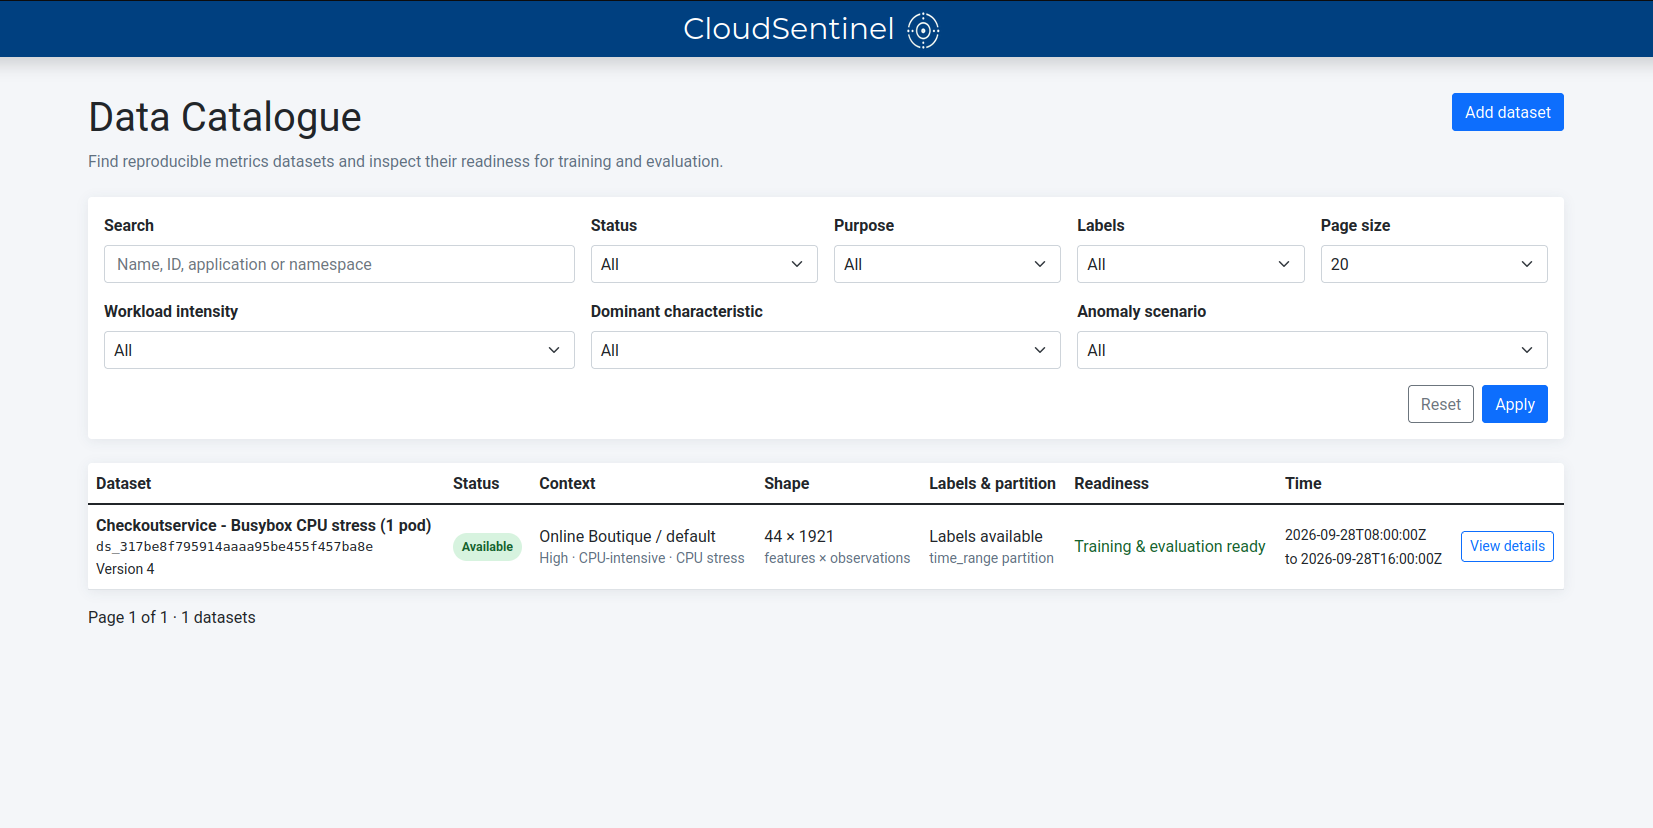
\includegraphics[width=0.95\linewidth]{figures/implementation/data_catalogue/Screenshot from 2026-10-06 17-18-47.png}
    \caption{The implemented Data Catalogue reports dataset identity, context, shape, labels, partitioning, and readiness.}
    \label{fig:condensed_data_catalogue_ui}
\end{figure}

Two supporting routes extend the basic Prometheus workflow. The CSV importer allows published or externally collected data to enter the same internal dataset contract. The Controlled Workload page can temporarily change the Online Boutique load-generator settings and records the actual start and end time before linking to dataset creation. The latter is intentionally limited to a small number of bounded traffic profiles and is not described as a general fault-injection platform.

\subsection{Detector integration, training, and Saved Models}

The training implementation supports several detector types through a shared plugin contract. A detector package contains a manifest and an adapter. The manifest provides the detector identity, version, supported modality, input requirements, capabilities, configurable parameters, and Python entry point. The same manifest is used by the backend for validation and by the interface for detector descriptions and parameter fields. This allows a compatible detector to appear in the existing workflow without adding a new training page or detector-specific HTTP route.

The adapter owns behaviour that cannot be made generic: detector-specific input checks, preprocessing, model fitting, evaluation, and the contents of the saved artefact. It implements methods for training and, when supported, for loading a model and producing inference predictions. CloudSentinel remains responsible for run states, progress, failure handling, verified input, artefact publication, and provenance. In this study, CGNN, Isolation Forest, and Local Outlier Factor use this contract. CGNN stores its fitted scaler and sequence configuration with the model. Isolation Forest and Local Outlier Factor store the fitted standardisation and estimator together as one pipeline.

External plugins are trusted server-side code. The Add detector page accepts a manifest, adapter, pinned dependency declaration, and optional supporting modules, but publication requires an operator key. Validation checks the package structure, manifest, declared methods, paths, and availability of the requested dependencies. Publication never installs packages into the running service. A valid package becomes an immutable versioned release and is only made available to new Training Runs after explicit activation. Existing runs keep the exact detector release that they originally selected.

A Training Run starts from one exact catalogue version and partition. The Learning service verifies the materialised bundle and creates one immutable snapshot. It then stores a parent run with one independent child for every selected detector. All children use the same snapshot and feature order, while each child receives its own validated parameters and pinned plugin release. A failure in one child does not remove a successful result from another child. The parent can therefore finish with complete success, failure, or partial success.

The worker loads the selected adapter only when its child starts. The adapter validates the snapshot, applies its preprocessing, fits and evaluates the detector, and writes its model files inside an assigned private workspace. CloudSentinel checks the returned files, records their checksums, and atomically publishes the artefact. Only then is a Saved Model record created.

A Saved Model is not only a model filename. It identifies the detector and plugin release, Training Run, dataset version, partition, snapshot checksum, feature-order hash, parameters, evaluation summary, model format, and artefact checksum. A model is marked inference-ready only when the runtime has enough information to verify and load its immutable artefact. Older or incomplete records may remain readable without being silently treated as usable for inference.

Figure~\ref{fig:condensed_training_ui} combines two representative parts of the implementation. The Detector Library is generated from validated manifests. The Training Run view shows the shared dataset evidence and the independent result of each detector child. Detailed wizard steps, manifest fields, and operator instructions are kept in the versioned project documentation rather than repeated in the thesis.

\begin{figure}[H]
    \centering
    \begin{subfigure}[t]{0.48\linewidth}
        \centering
        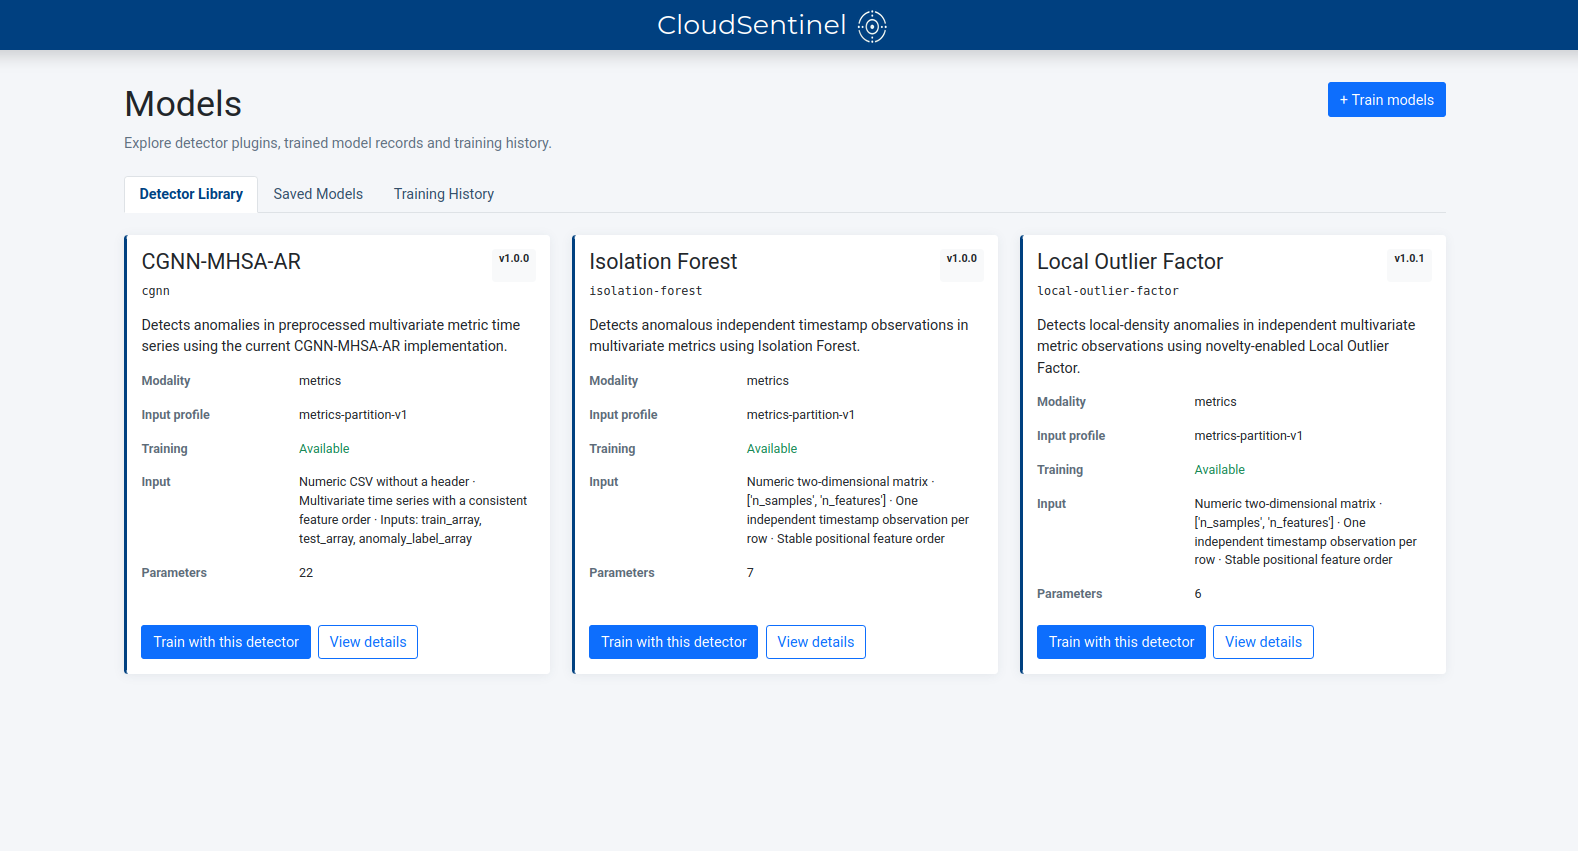
\includegraphics[width=\linewidth]{figures/implementation/Models_and_training/Screenshot from 2026-10-06 17-24-06.png}
        \caption{Detector Library generated from plugin manifests.}
    \end{subfigure}\hfill
    \begin{subfigure}[t]{0.48\linewidth}
        \centering
        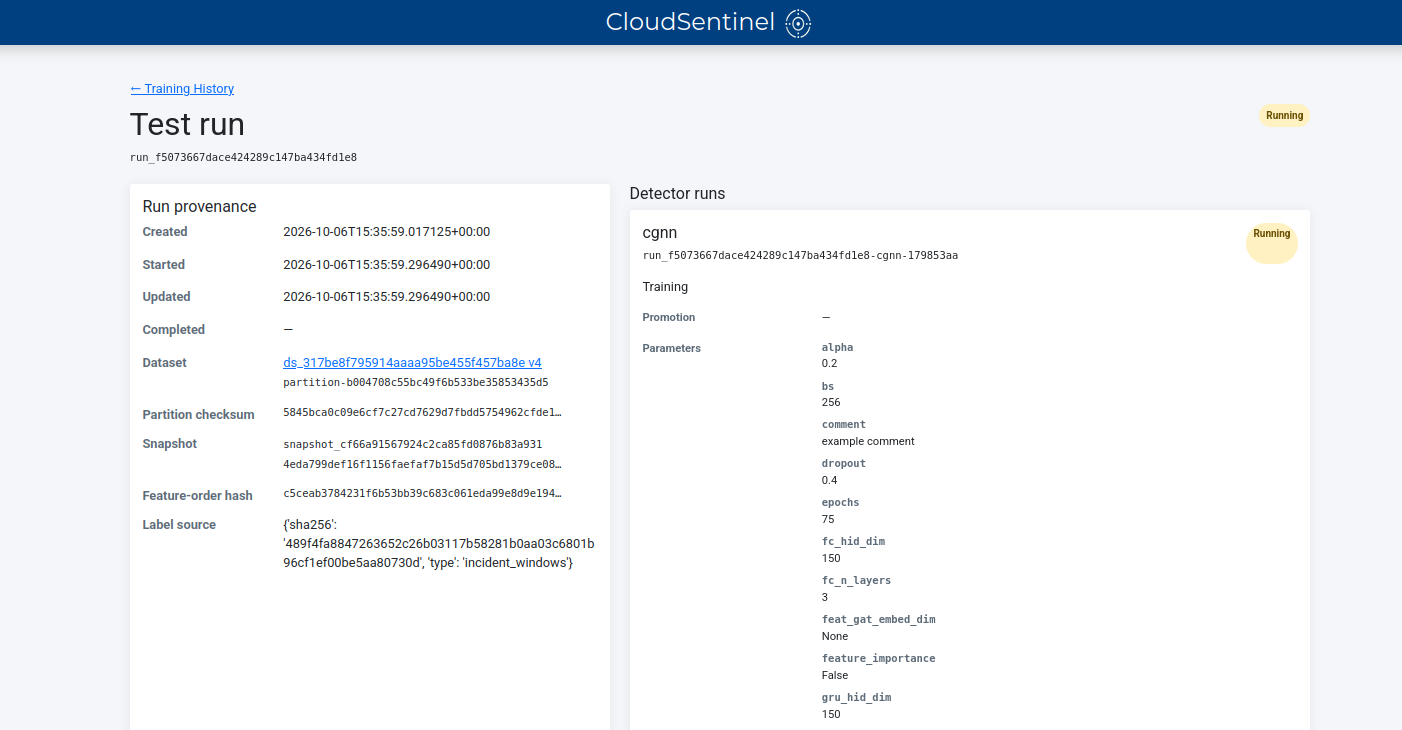
\includegraphics[width=\linewidth]{figures/implementation/Models_and_training/training_workflow/Screenshot from 2026-10-06 17-37-54.png}
        \caption{Training Run with shared input and per-detector results.}
    \end{subfigure}
    \caption{Representative detector-management and training views.}
    \label{fig:condensed_training_ui}
\end{figure}

This implementation separates reproducibility from physical parallelism. Detector children have independent records and failure handling, but the evaluated staging deployment may still execute them sequentially because it uses a limited number of workers. The plugin contract also improves extensibility without sandboxing arbitrary Python code. External detector implementations must therefore come from a trusted developer or operator.

\subsection{Model Comparisons and Robustness}

A Model Comparison evaluates at least two concrete Saved Models on the same catalogue test partition. It compares trained artefacts rather than detector names: two models produced by separate Training Runs are different candidates even when they use the same detector algorithm. Conversely, the same exact Saved Model can be evaluated again in another workload context.

Before a comparison is created, the Learning service checks that every selected model is available, inference-ready, and compatible with the evaluation data. The model and dataset must use the same modality and exact feature identity. The final request pins the dataset version, partition checksum, workload context, feature-order hash, Saved Model identifiers, and artefact-manifest checksums before the worker starts. A later model or dataset change cannot silently alter the queued comparison.

The worker requests a verified evaluation bundle from the Data Catalogue and sends its matrix to the Generic Detection Runtime once for each selected Saved Model. The runtime loads the exact model artefact through its adapter and returns predictions, anomaly scores, warm-up count, runtime, and identifying hashes. CloudSentinel verifies these values before calculating and storing the available comparison measures. Failure of one model produces a partial comparison when other models complete successfully.

When ground-truth labels are present, the result includes the confusion-matrix counts, precision, recall, and F1. Precision describes the fraction of predicted anomalies that were actually anomalous. Recall describes the fraction of labelled anomalies that were detected. F1 balances these two values. These measures are unavailable rather than invented when labels are missing.

Sequence models may require earlier observations before their first valid prediction. The runtime reports this as the warm-up count, and CloudSentinel aligns the labels and timestamps with the remaining predictions. Detection lead time is calculated from the first valid predicted anomaly to the start of the known incident. A detection after incident start is reported as late rather than being presented as a negative lead time with an unclear meaning.

Each completed Comparison Run contains five views: an overview, timeline, model details, experiment evidence, and robustness. The Experiment Evidence view records what produced the scores: the exact dataset partition, workload context, features, Saved Models, detector releases, and originating Training Runs. Figure~\ref{fig:condensed_comparison_ui} shows this evidence beside the cross-context robustness view.

\begin{figure}[H]
    \centering
    \begin{subfigure}[t]{0.48\linewidth}
        \centering
        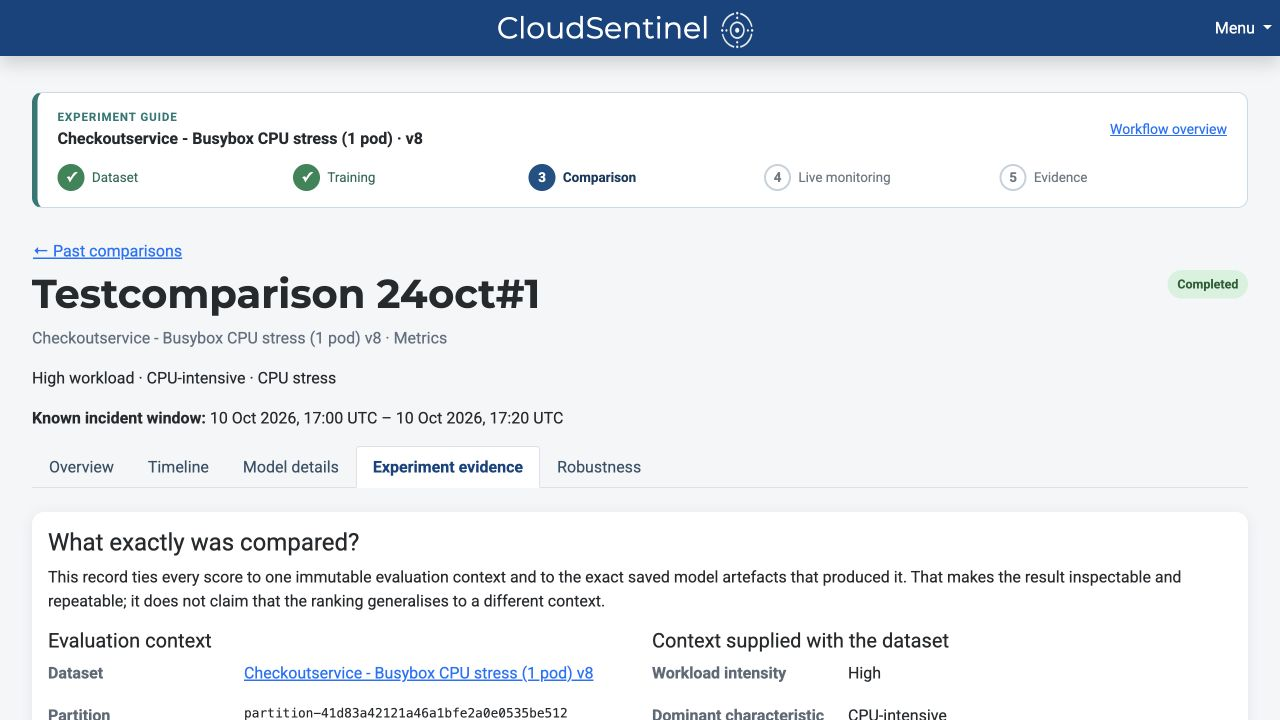
\includegraphics[width=\linewidth]{figures/implementation/current/comparison_evidence.jpg}
        \caption{Evidence for one comparison context.}
    \end{subfigure}\hfill
    \begin{subfigure}[t]{0.48\linewidth}
        \centering
        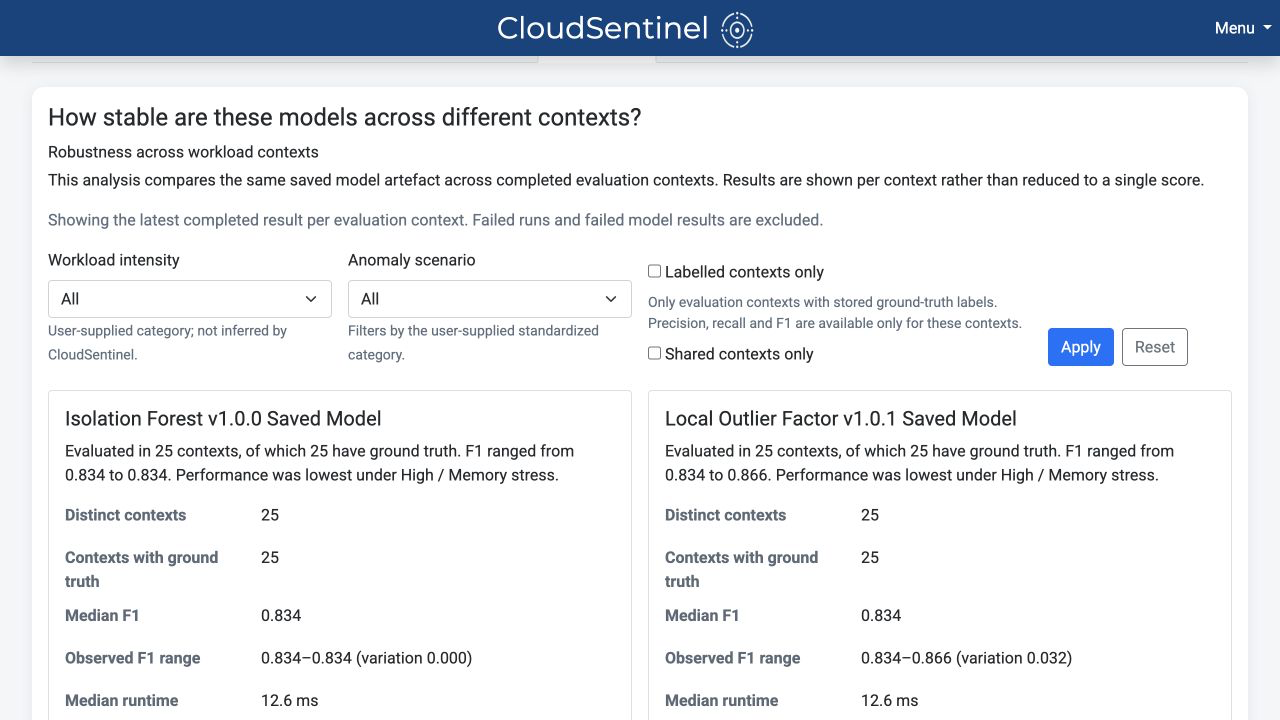
\includegraphics[width=\linewidth]{figures/continued_context_evaluation.png}
        \caption{The same artefacts across multiple contexts.}
    \end{subfigure}
    \caption{Comparison provenance and historical robustness for exact Saved Model artefacts.}
    \label{fig:condensed_comparison_ui}
\end{figure}

One Comparison Run only provides evidence for one evaluation context. The Robustness view therefore finds earlier completed results for the same exact artefact, identified by its model identifier, artefact identifier, and manifest checksum. Repeated runs on the same partition are deduplicated so that a retry does not look like another independent context. Unlabelled contexts can contribute runtime coverage but not precision, recall, or F1.

For each model, the view reports context coverage, labelled coverage, median F1, observed F1 range, median precision and recall, runtime, and lead-time coverage. Direct comparisons are restricted to contexts shared by the selected artefacts. CloudSentinel does not combine these measures into one general robustness score. A statement about the lowest observed variation is only made when every selected artefact has valid F1 evidence in at least two of the same contexts.

The result page also offers goal-based decision support for the current context. A user can prioritise F1, recall, precision, valid lead time, or measured inference runtime. The recommendation is a read-only ordering of available results and explicitly applies only to the selected dataset and workload context. It does not activate or promote a model automatically. The same exact models can be carried into another comparison so that additional robustness evidence can be collected without finding them again manually.

\subsection{Live Monitoring and monitoring history}

The original Live Monitoring path was tied to CGNN-specific routes. The revised path starts from one explicit Saved Model and its stored input recipe. A newly collected Prometheus dataset records a live-input recipe containing the source identifier, executed queries, targets, series-to-feature mapping, sampling interval, feature order, and missing-value policy. Its checksum and feature hash are carried through training into the Saved Model. CloudSentinel does not guess a live query from a model name or feature label.

When a session starts, Data Ingestion pins the model, artefact, recipe, and feature hashes. The worker executes only the stored queries against the centrally configured Prometheus source and reconstructs the input in the expected feature order. A matrix with missing values is rejected rather than silently filled, because imputation could change the model result. The Generic Detection Runtime then loads the exact model through its detector adapter. Detector-specific scaling, sequence construction, warm-up, and prediction use the same artefact information that was stored during training.

A monitoring session consists of separate cycles. Each cycle has a Prometheus query window, an inference window, and a prediction window. The inference window may repeat earlier observations to give a sequence model enough context, but a prediction watermark ensures that only new timestamps are committed. This prevents overlapping Prometheus windows or task retries from counting the same prediction twice.

The displayed anomaly percentage is the number of anomalous new predictions divided by all new predictions in that cycle. Warm-up and cycles without new data have no percentage; the interface labels them explicitly instead of displaying zero. The input, result, warnings, checksums, model identity, and timing are committed to durable history before the cycle appears in the interface. Earlier evidence therefore remains available after the temporary Redis task state expires.

Figure~\ref{fig:condensed_monitoring_ui} shows the setup and history views. Setup contains the model, cycle timing, and optional RCA choices. History retains session state, model provenance, a chart of valid cycle summaries, and links to the stored evidence. Stopping a session is written to durable storage before worker cancellation is attempted, so a late worker cannot append another cycle after the stop.

\begin{figure}[H]
    \centering
    \begin{subfigure}[t]{0.48\linewidth}
        \centering
        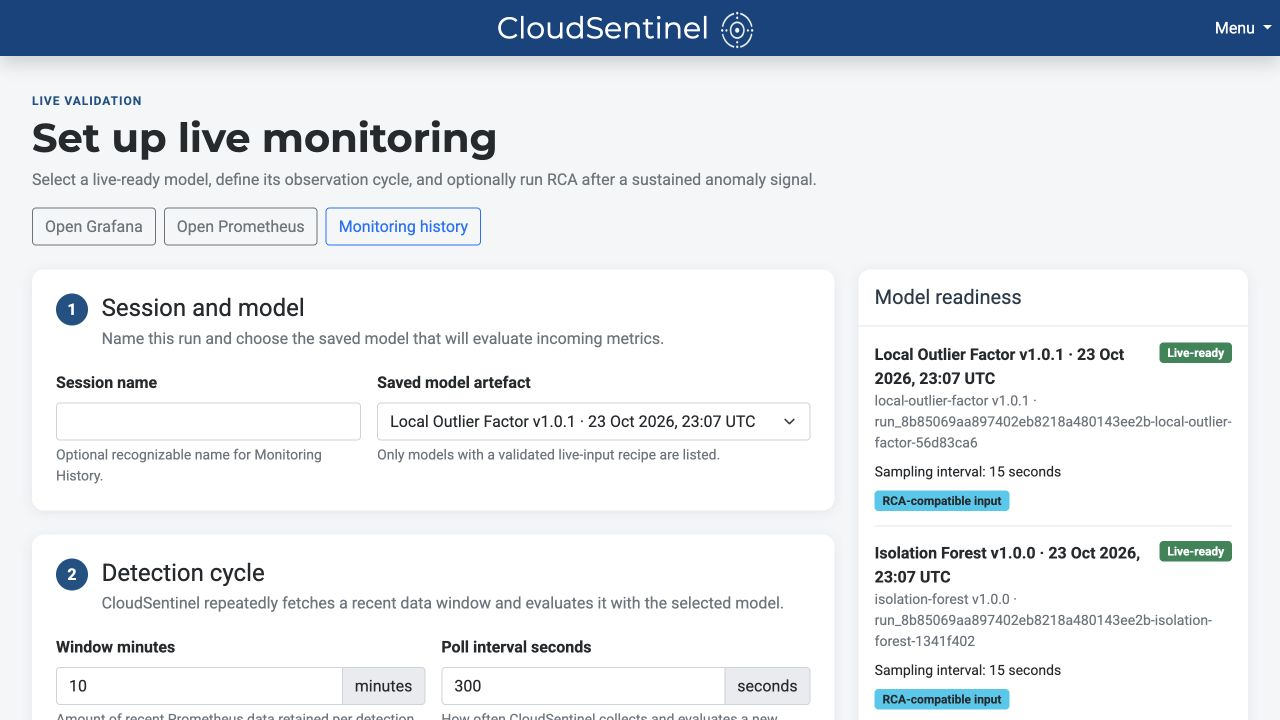
\includegraphics[width=\linewidth]{figures/implementation/current/monitoring_setup.jpg}
        \caption{Monitoring Setup.}
    \end{subfigure}\hfill
    \begin{subfigure}[t]{0.48\linewidth}
        \centering
        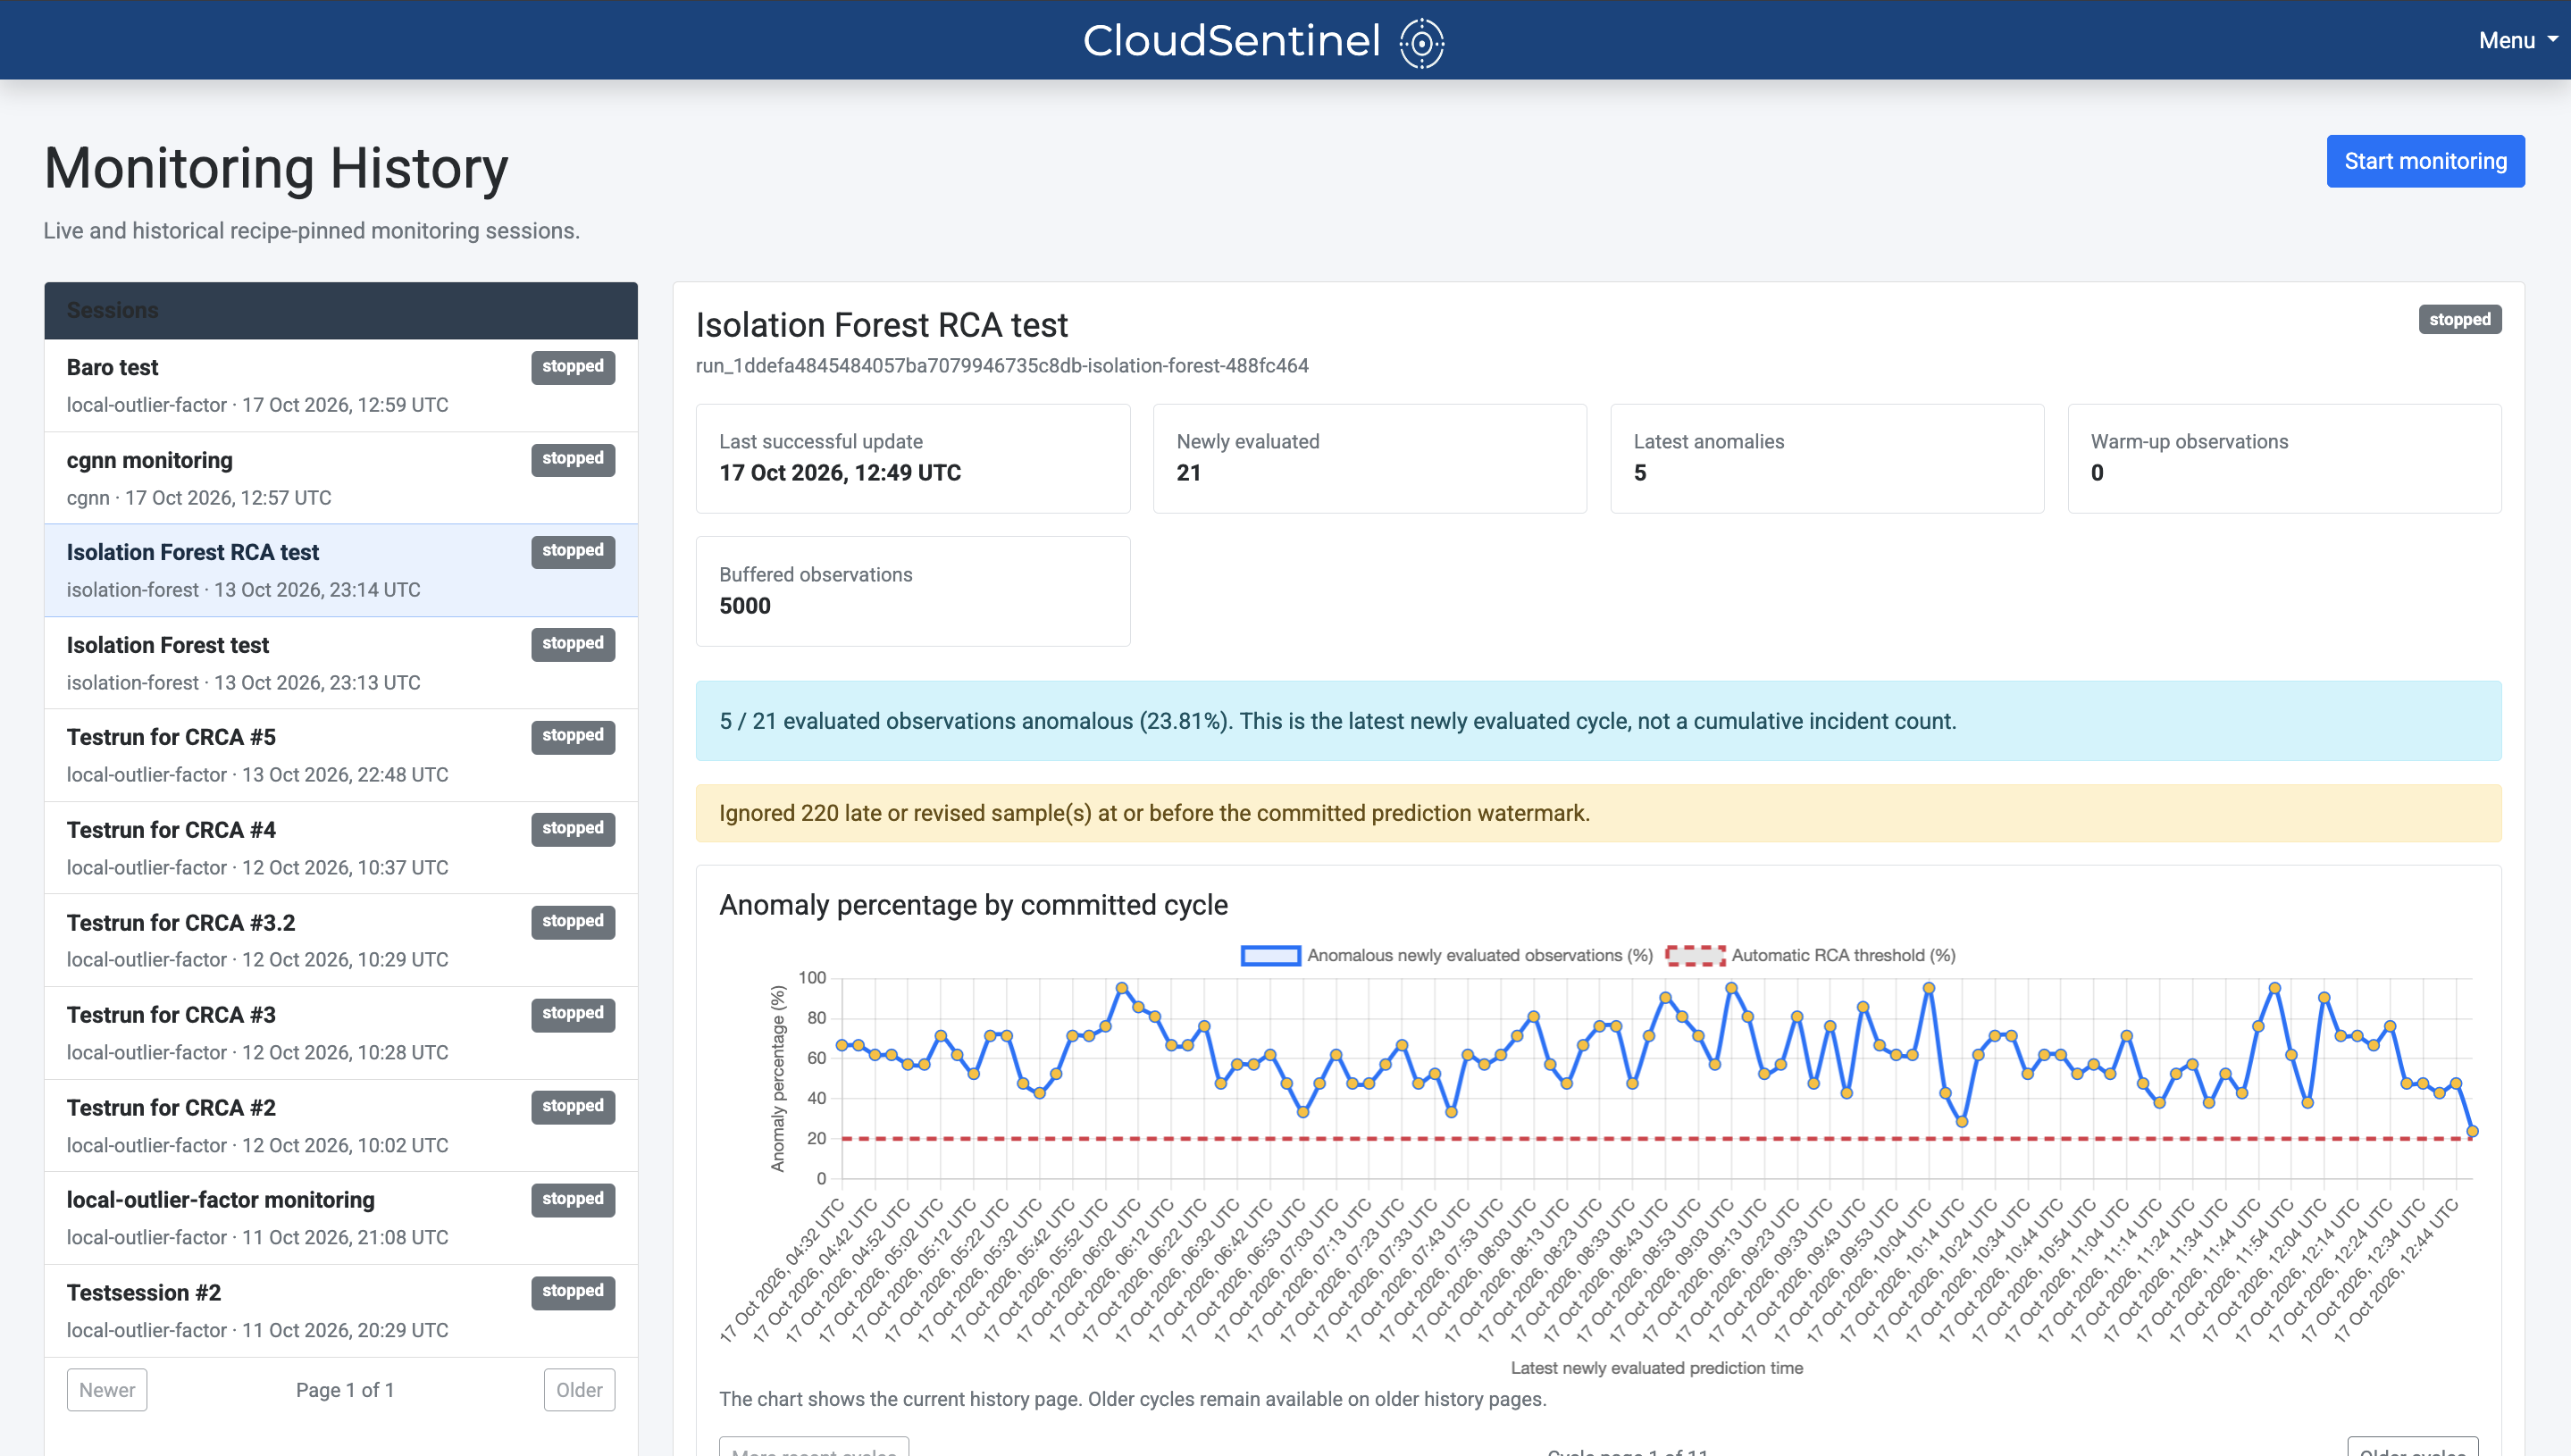
\includegraphics[width=\linewidth]{figures/implementation/extra/Screenshot 2026-10-18 at 23.17.08.png}
        \caption{Durable Monitoring History.}
    \end{subfigure}
    \caption{Live Monitoring uses an exact Saved Model and stores its completed cycles as revisitable evidence.}
    \label{fig:condensed_monitoring_ui}
\end{figure}

\subsection{Selectable root-cause analysis}

RCA is connected to a successfully committed monitoring cycle. It is optional and remains separate from anomaly detection: a detector can be live-ready while its input is unsuitable for an RCA method, and an RCA failure does not stop the monitoring session. A run is considered only when a cycle contains new predictions and its anomaly percentage is strictly above the configured threshold.

CloudSentinel selects the RCA window from the checksummed input already stored for the triggering cycle. It does not perform another Prometheus query that might return different data. The method, configuration, model and recipe identities, analysis window, and input checksum form the stable run identity. The session also stores episode state. Continued high cycles normally belong to the same episode and do not create unlimited RCA tasks. A later analysis can only be accepted after recovery or when bounded same-episode reanalysis conditions are met.

The evaluated implementation provides two method contracts. CausalRCA receives finite multivariate observations and can return a feature ranking and dependency graph. BARO RobustScorer compares a baseline segment with the period after the first stored positive anomaly prediction. It returns a ranking and change-point evidence but no causal graph. Scores are relative within one run; they are not probabilities and cannot be compared directly between methods.

Before execution, Data Ingestion writes a durable intent containing the trigger decision and pinned evidence. The CRCA worker claims that intent, loads the private input, executes the method adapter, validates its output, and stores a checksummed result. Monitoring History distinguishes completed, failed, skipped, and suppressed analyses. The result contains the method, trigger, time window, input source, bounded ranking, optional graph, and safe failure reason.

\begin{figure}[H]
    \centering
    \begin{subfigure}[t]{0.48\linewidth}
        \centering
        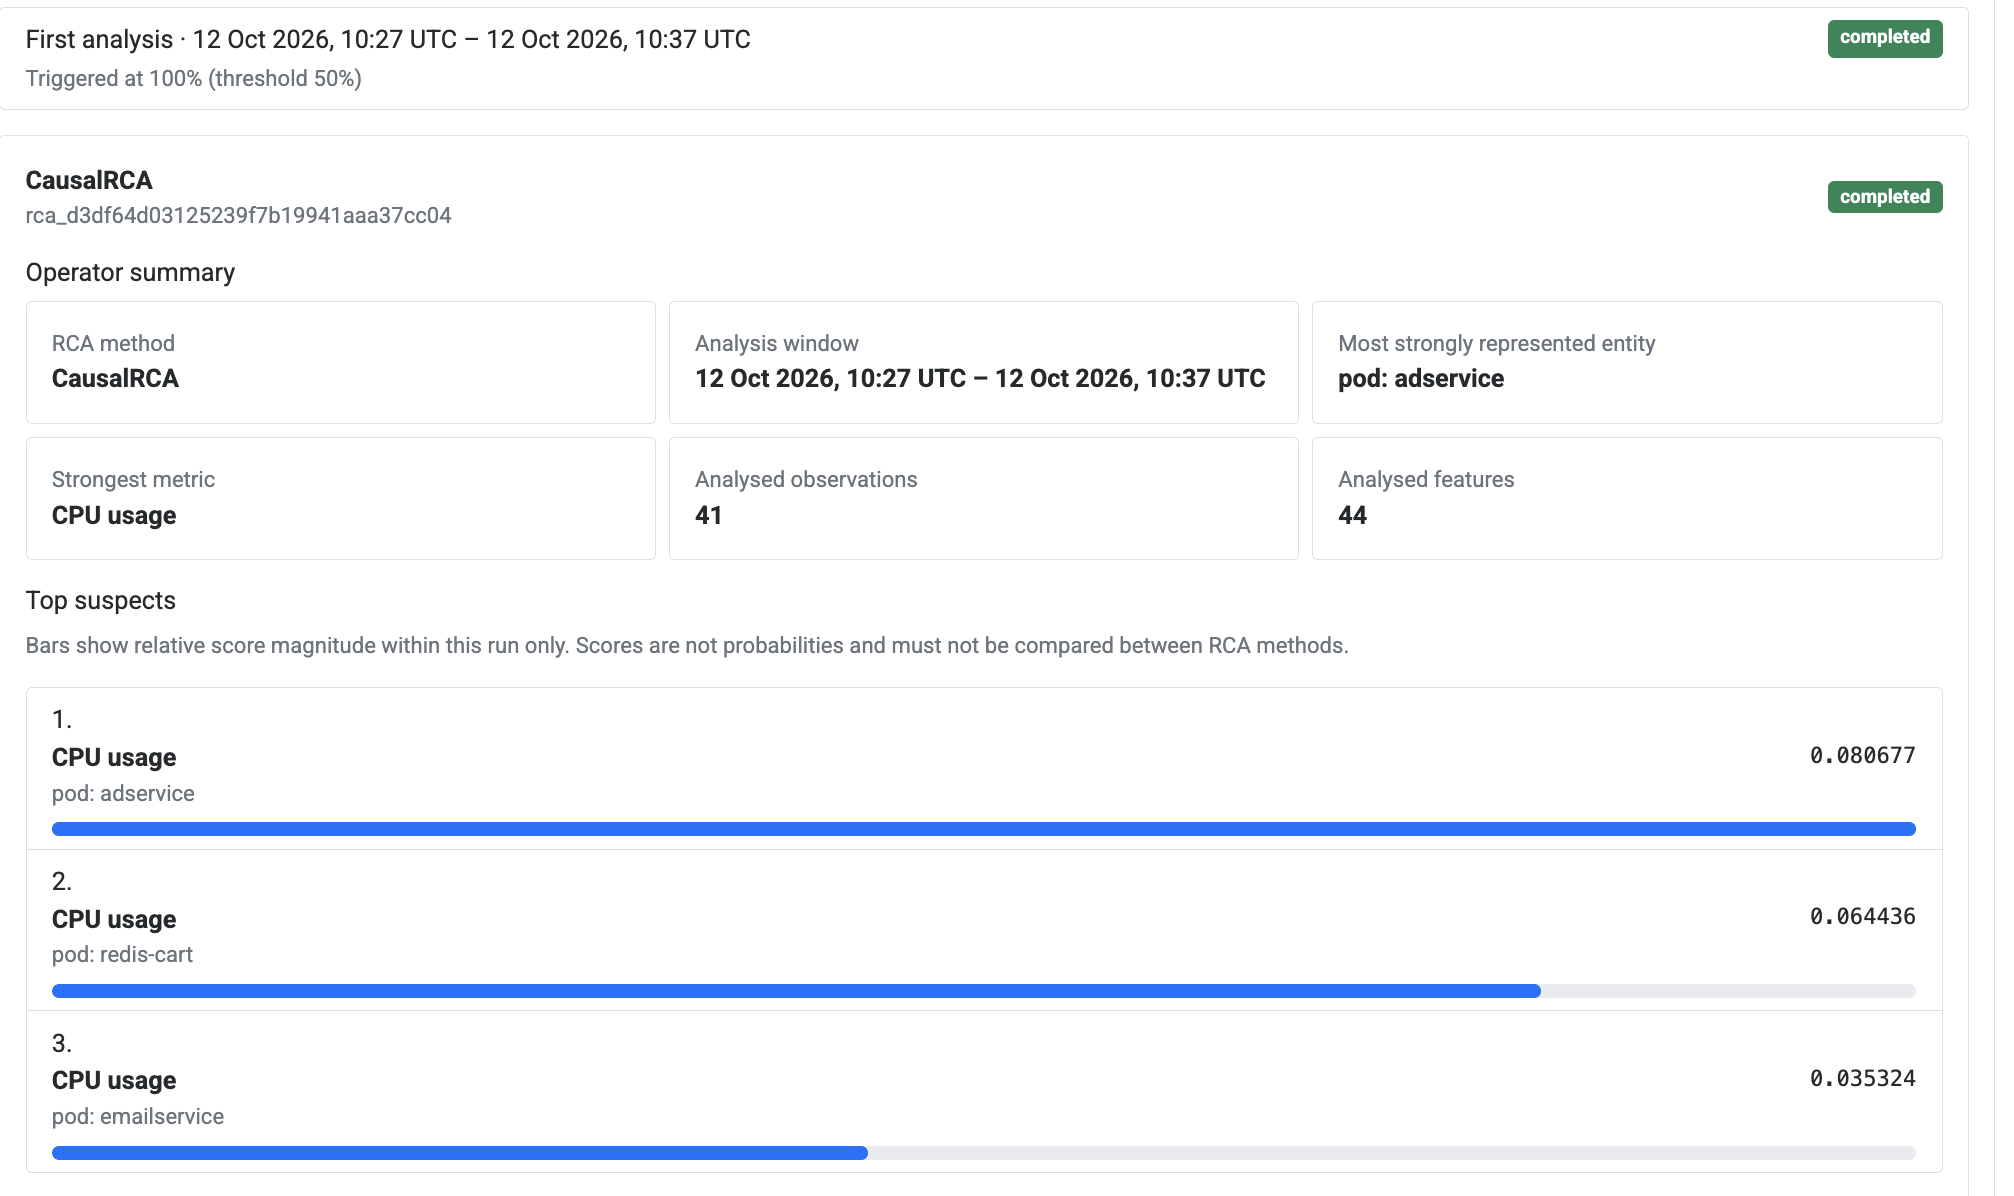
\includegraphics[width=\linewidth]{figures/implementation/extra/Screenshot 2026-10-18 at 23.19.27.png}
        \caption{Stored method and trigger information.}
    \end{subfigure}\hfill
    \begin{subfigure}[t]{0.48\linewidth}
        \centering
        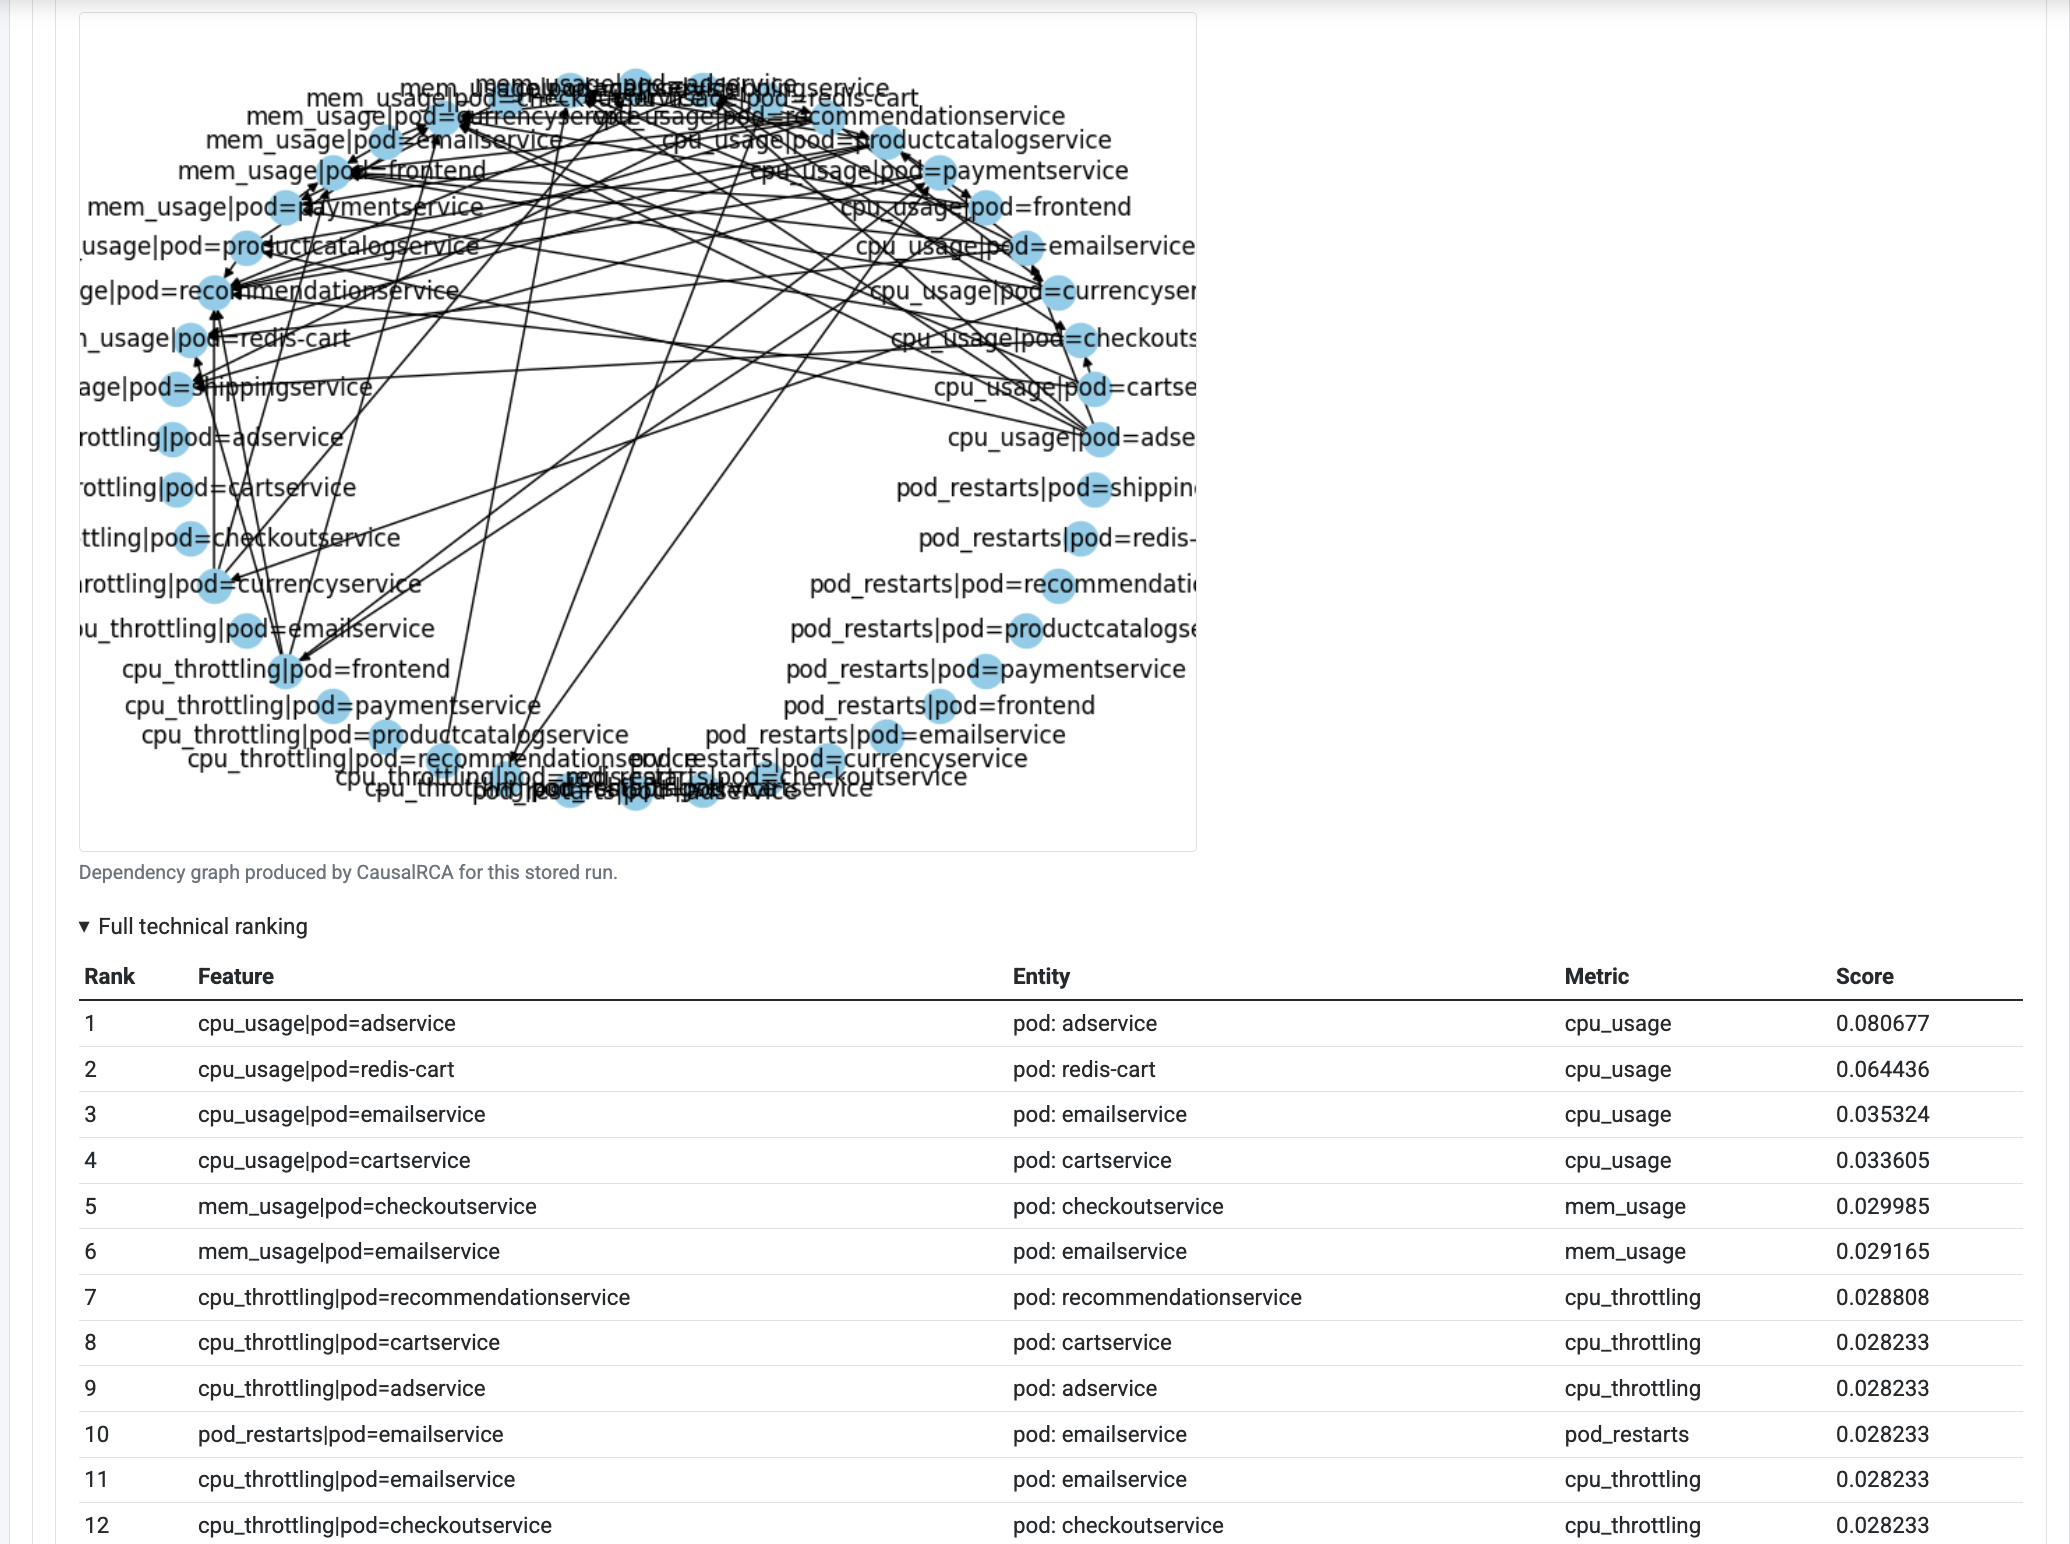
\includegraphics[width=\linewidth]{figures/implementation/extra/Screenshot 2026-10-18 at 23.19.45.png}
        \caption{Bounded ranking and provenance.}
    \end{subfigure}
    \caption{A stored RCA result retains both the diagnostic output and the evidence needed to interpret it.}
    \label{fig:condensed_rca_ui}
\end{figure}

The interface describes an RCA result as diagnostic evidence. A top-ranked feature is not automatically the actual root cause, and a calculated dependency is not proof of causality. The redesign improves repeatability and inspection of the analysis, but operator interpretation remains necessary.

\subsection{Implementation boundaries and supporting documentation}

The implementation was built for the controlled single-node Kubernetes environment used in this study. The API services and workers use shared persistent volumes and process-level file locks. Atomic replacement and checksums protect the tested workflow against partial writes and changed files, but they do not provide distributed transactions. A multi-node production deployment would require storage that supports multiple writers, distributed coordination, indexed records, retention policies, and stronger recovery from workers that remain in an uncertain state.

Detector plugins also remain trusted code. The manifest and publication process make their requirements and identity explicit, but they do not sandbox Python. New dependencies require a planned runtime-image update. Release signing, automatic removal of unused plugin releases and model artefacts, and automatic retention of monitoring and RCA evidence are outside the implemented scope.

The implementation uses metrics as its telemetry modality. The plugin and dataset records expose a modality field, but logs and traces are not carried through the complete workflow. Comparison execution is bounded and sequential inside one worker task, and the measured runtime is not a proof of horizontal scalability. These limits are important when interpreting the evaluation later in this chapter.

Detailed operational instructions are maintained separately from the manuscript. The project repository contains versioned documentation for the Data Catalogue, detector registry and external-plugin contract, Training Runs, Generic Detection Runtime, Model Comparisons and Robustness, Live Monitoring, RCA, deployment, and known limitations. The documentation version corresponding to this manuscript is available at \url{https://github.com/ThomasGITH/fork_cloudsentinel/tree/89222d9cc3a08c2e77c602eb0a2f5516f6db8e44/docs}. Keeping step-by-step fields and installation instructions there allows the thesis to focus on the implemented research contribution while preserving the technical details needed to operate or extend the prototype.

\subsection{Terms used in the evaluation}

Table~\ref{tab:evaluation_terms} summarises the main implementation terms used in the following evaluation. It is included here so that the evaluation can be read without remembering every implementation detail.

\begin{table}[H]
    \centering
    \caption{Main CloudSentinel terms used in the evaluation.}
    \label{tab:evaluation_terms}
    \begin{tabularx}{\linewidth}{@{}p{34mm}X@{}}
        \toprule
        \textbf{Term} & \textbf{Meaning in the implemented workflow} \\
        \midrule
        Dataset Version & One fixed collection or import with a source, feature order, files, context, and checksums. \\
        Dataset Partition & The explicit training and test selection stored for one Dataset Version. \\
        Detector Plugin & A versioned manifest and adapter that connect one detector implementation to the shared training and inference contracts. \\
        Training Run & One stored training request containing a shared dataset snapshot and an independent child result for every selected detector. \\
        Saved Model & An available trained model record linked to its dataset, Training Run, detector release, parameters, feature identity, and immutable artefact. \\
        Model Comparison & A stored evaluation of at least two compatible Saved Models on the same dataset test partition. \\
        Workload Context & User-supplied categories that describe the circumstances and anomaly scenario represented by a dataset. \\
        Monitoring Session & Repeated live detection cycles using one exact Saved Model and its stored Prometheus input recipe. \\
        Monitoring Cycle & One committed collection and inference step containing only the newly accepted predictions and their evidence. \\
        RCA Result & A stored diagnostic analysis linked to its triggering cycle, method, time window, checksummed input, ranking, and optional graph. \\
        \bottomrule
    \end{tabularx}
\end{table}

